%
% حق نشر 1390-1402 دانش پژوهان ققنوس
% حقوق این اثر محفوظ است.
% 
% استفاده مجدد از متن و یا نتایج این اثر در هر شکل غیر قانونی است مگر اینکه متن حق
% نشر بالا در ابتدای تمامی مستندهای و یا برنامه‌های به دست آمده از این اثر
% بازنویسی شود. این کار باید برای تمامی مستندها، متنهای تبلیغاتی برنامه‌های
% کاربردی و سایر مواردی که از این اثر به دست می‌آید مندرج شده و در قسمت تقدیر از
% صاحب این اثر نام برده شود.
% 
% نام گروه دانش پژوهان ققنوس ممکن است در محصولات دست آمده شده از این اثر درج
% نشود که در این حالت با مطالبی که در بالا اورده شده در تضاد نیست. برای اطلاع
% بیشتر در مورد حق نشر آدرس زیر مراجعه کنید:
% 
% http://dpq.co.ir/licence
%
% TODO: maos 1391: استفاده از یک بسته نرم‌افزاری دیگر
% از بسته‌های نرم‌افزاری برای توصیف فرآیند استفاده شده است. با استفاده از بسته‌های
% متفاوت می‌توان محصولات خودمان را نیز معرفی کنیم.

\section{\lr{OBS}}

سرویس ساخت \lr{OpenSUSE}\LTRfootnote{Opne Build Service} که با نام اختصاری
\lr{OBS} نمایش دهده می شود یک سکوی توسعه گسترده است. در این سکوی توسعه امکان‌های پایه‌ای مورد
نیاز برای ساخت پروژه‌های متن باز برای سیستم‌عامل‌های لینوکس را فراهم کرده است.
در این سکوی توسعه امکان ایجاد یک سیستم نه تنها بر اساس توزیع‌های متفاوت لینوکس
فراهم شده است بلکه امکان ایجاد بر اساس معماری‌های متفاوت نیز وجود دارد. در حال
حاضر این سرور باز ساخت پروژه‌های متن باز به بیش از 30000 کاربر خدمات داده و بیش
از 160000 بسته را برای معماری‌ها و سیستم‌های عامل متفاوت فراهم کرده
است\cite{buildopensuse}.

% What exactly is the Open Build Service ?

\lr{OBS} در حقیقت محیط توسعه‌ای است که ابزارهای مورد نیاز توسعه دهندگان
پروژه‌های متن باز در فرآیند ایجاد را فراهم کرده است. با استفاده از این ابزار
می‌توان به سادگی پروژه‌های متن باز را نه تنها برای توزیع‌ها متفاوت لینوکس بلکه
برای معماری‌های متفاوت ایجاد کرده و برای استفاده دیگر کاربران آن را به اشتراک
گذاشت.

بزرگترین ایرادی که می‌توان به نرم‌افزارهای توسعه داده شده برای لینوکس وارد کرد،
عدم کاربرد بسته‌های ایجاد شده برای یک توزیع از این سیستم عامل در توزیع‌های دیگر
است. به بیان دیگر زمانی که یک توسعه دهند یک بسته نرم‌افزاری را برای یک توزیع خاص
از لینوکس ایجاد می‌کند (برای نمونه \lr{ReadHat}) در بسیاری از موارد نمی‌توان آن
را برای توزیع‌های دیگر به کار برد.

کارگزار ساخت \lr{OpenSUSE} تنها کارگزار متن بازی است که امکان ایجاد بسته‌های
نرم‌افزاری را در یک زمان برای توزیع‌های متفاوت لینوکس و تمام
ابزارهای مورد نیاز در این فرآیند را به بهترین شکل  فراهم کرده است.

%  With the system imaging tool
% KIWI, open source developers can more quickly build a Linux distribution that
% meets their needs, rigorously test it to ensure product quality, and easily
% package it for quick installation. Users can easily find the latest open source
% packages they are looking for and will be able in the future to build customized
% distributions.
%
% The Open Build Service is completely open source, giving developers and users
% free and full access to build their choice of Linux packages, whether they are
% based on openSUSE, SUSE Linux Enterprise, Fedora, Debian, Ubuntu or other
% projects.

% Can anybody build packages with the Open Build Service ?

برای ایجاد یک پروژه به روی این کارگزار به آدرس آن (\lr{build.opensuse.org})
مراجعه کرده و یک  کاربر ایجاد کنید. با استفاده از این کاربر می‌توان پروزه‌های متن باز را ایجاد کرده و
مبتنی بر آنها مخزن نرم‌افزاری برای توزیع‌های متفاوت لینوکس ایجاد کرد.

این کارگزار ساخت نه تنها با استفاده از واسط تارنما بلکه با استفاده از برنامه‌های
کاربردی متفاوت قابل دسترسی است. در تارنمای این کارگزار فهرست تمام پروژه‌های
موجود بوده و گزارش کاملی از وضعیت جاری کارگزار نمایش داده شده است. در این تارنما
راهنمای کامل کاربری ایجاد شده است که کاربران را در استفاده از آن یاری می‌کند.


%
% But bear in mind that the Open Build Service is a community support project. So
% please, if you plan to build packages, make sure
%
%     your package really adds something new to the community
%     you talk to people that are working on similar packages or topics
%     to rather help on existing packages than duplicating packages
%     you let people know about what you're doing to find other interested community members. Mailinglists are the right place to do that.
%
% Always remember, regardless how much build power is added to the build service,
% it can be eaten up by not so usefull packages ;-)


% Can the Open Build Service build package for other distributions ?

گرچه در هنوز در این کارگزار ساخت، سیستم‌عامل‌هایی مانند مک\LTRfootnote{Mac} و
یا ویندوز حمایت نمی‌شود اما امکان ساخت بسته‌های نرم‌افزاری در قالب‌های
\lr{RPM}\LTRfootnote{Read Hat Package Manager} و \lr{debian} وجود دارد. در این
کارگزار توزیع‌های \lr{Debian}، \lr{Ubuntu}، \lr{Fedora}، \lr{CentOS} و
\lr{Mandriva} به صورت مستقیم مورد حمایت قرار می‌گیرد.


% Can I build my own distribution with the Open Build Service ?
%
% KIWI, used by the Build Service, supports the generation of image files.
% openSUSE 11.2 was produced completely using the Build Service, including images.
% For an example of customising the distribution, look at the KDE:Medias project,
% which offers stable openSUSE updated with the most recent KDE release.

% Why is the Open Build Service unique ?
این کارگزار ساخت یکی از کارگزاران ساخت نرم‌افزاری منحصر به فرد به شمار می‌رود.
برخی از خصوصیت‌های این کارگزار ساخت که آن را به یک نمونه منحصر به فرد تبدیل کرده
است عبارت است از:

\begin{itemize}
  \item می‌یابد این کارگزار کاملا متن باز توسعه.
  \item این کارگزار فرآیند ایجاد بسته‌های نرم‌افزاری را بسیار ساده کرده است.
  \item با استفاده از این کارگزار می‌توان بسته‌ها را به صورت عملی مورد آزمون
  قرار داد.
  \item این روش بهترین رویکرد برای ایجاد مخزن‌های بزرگ نرم‌افزاری است.
  \item با استفاده از آن می‌توان بسته‌های نرم‌افزاری را برای توزیع‌های متفاوت از
  لیونکس ایجاد کرد.
  \item این کارگزار واسط بسیار ساده کاربری برای نصب بسته‌های نرم‌افزاری ایجاد
  کرده است.
  \item یک پارچگی سیستم همواره حفظ می‌شود به این معنی که اگر یک بسته مورد
  استفاده در سیستم تغییر کرد، بسته‌های وابسته به صورت خودکار ترجمه و ایجاد
  می‌شوند.
\end{itemize}

گرچه با استفاده از واسط تارنمای این کارگزار ساخت کاربران به سادگی قادر خواهند
بود فرآیند ایجاد سیستم‌های نرم‌افزاری را مدیریت کنند اما امکان استفاده از خط
فرمان در فرآیند ساخت نیز فراهم شده است. با استفاده از بسته نرم‌افزاری \lr{osc}
که برای بسیاری از توزیع‌های لینوکس موجود است، کاربران قادراند با استفاده از خط
فرمان فرآیند ایجاد سیستم نرم‌افزاری خود را مدیریت کنند.

گرچه تارافزار این کارگزار روشی بسیار ساده برای مدیریت فرآیند ساخت را فراهم کرده
است اما با استفاده از خط فرمان می‌توان فرآیند ساخت را به صورت محلی اجرا کرده و
خطاهای موجود در فرآیند ساخت را شناسایی و رفع کرد. بسته \lr{osc} محیط ساخت
بسته نرم‌افزاری را به روی رایانه نصب کرده و کاربران را قادر می‌سازد که نه تنها
فرآیند ساخت بلکه رفع خطای این فرآیند را به روی رایانه شخصی خود اجرا کنند که یک
روش بسیار مناسب برای آموزش، رفع خطا و بررسی صحیت فرآیند ساخت است.

\subsection{پروژه}

در این کارگزار ساخت معادل با هر کاربر یک پروژه ایجاد می‌شود که هم نام با نام
کاربری است. پروژه در اینجا به معنی یک گردایه از بسته‌های نرم افزاری است که با یک
دیگر یک یا چند مخزن نرم‌افزاری را سازماندهی می‌کنند. برای نمونه فرض کنید که یک
مخزن از بسته‌های نرم‌افزاری مورد استفاده در رمزنگاری موجود است. تمام این
بسته‌های نرم‌افزاری را می‌تواند در قالب یک مخزن نرم‌افزاری در نظر گرفته و به
صورت یک پروژه در این کارگزار مدیریت کرد. در این بخش پروژه به معنی موجودیتی در
نظر گرفته می‌شود که در این کارگزار تعریف شده است و مواردی که هدف تعریف دیگر از
پروژه باشد به آن اشاره خواهد شد.

پروژه اصلی ایجاد شده برای هر کاربر به عنوان پروژه خانه\LTRfootnote{Home Project}
در نظر گرفته می‌شود. این نام گذاری به این دلیل است که کاربران مجار به ایجاد
پروژه‌های دیگر خارج از پروژه اصلی خود نیستند از این رو پروژه اصلی هر کاربر 
پروژه خانه وی در نظر گرفته می‌شود.

در تارافزار این کارگزار گزینه‌های متفاوتی برای مدیریت پروژه‌ها وجود دارد که
امکان خصوصیت‌های متفاوتی از پروژه را فراهم کرده است. مهم‌ترین خصوصیت‌های قابل
تغییر در فهرست زیر آورده شده است.

\begin{itemize}
  \item گزار حالت کلی پروژه
  \item مدیریت بسته‌ها
  \item مدیریت مخزن نرم‌افزاری
  \item مدیریت نیازها
  \item مدیریت کاربران
\end{itemize}

با استفاده از گزارش‌های ایجاد شده می‌توان تعیین کرده که کدام بسته‌های نرم‌افزاری
ترجمه و یا کدام بسته‌ها در فرآیند ایجاد و بسته بندی با مشکل رو برو شده اند و یا
حتی تعیین کرد که بسته‌های مورد نظر برای کدام سیستم‌های عامل ایجاد و یا در حال
ساخت هستند. مدیریت بسته‌های امکان اضافه و مدیریت کردن بسته‌های نرم‌افزاری به
مخزن‌های ایجاد شده را فراهم می‌کند در حالی که مدیریت نیازها و کاربران امکان
تعیین نیازهای جدید در بسته‌ها و یا کاربران مجاز بسته‌های ایجاد شده را فراهم
می‌کند.

معادل با هر مخزن، در سیستم یک مکان در نظر گرفته می‌شود و نتایج به وجود امده از
فرآیند ساخت در آنها قرار گرفته می‌شود. از این رو با استفاده از ابزارهای مدیریت
بسته می‌توان به سادگی بسته‌های نرم‌افزاری را روی رایانه‌های مقصد نصب و به روز
رسانی کرد. از آنجا که هر پروژه نه تنها برای توزیع‌های متفاوت بلکه نسخه‌های
متفاوت ایجاد می‌شود نیاز است که مخزن‌های متفاوتی برای یک پروژه در نظر گرفت. از
این جهت مخزن در اینجا معادل با سکویی در نظر گرفته می‌شود که سیستم برای آن ایجاد
شده است. به این ترتیب در مدیریت مخزن‌ها، سیستم‌های عامل
هدف\LTRfootnote{Distance Machine} تعیین، و بیان می‌شود که بسته‌های ایجاد شده
برای هر سیستم عامل چه رفتاری باید داشته باشد.

در شکل  \ref{image/standard/build/opensuse-project-overview} یک نمایش از واسط
مدیریت پروژه نمایش داده شده است. همانگونه که در این شکل قابل مشاهده است علاوه بر
گزارش کلی فرآیند ساخت سامانه مناسب برای مدیریت پروژه در نظر گرفته شده است.

\begin{figure}
\centering
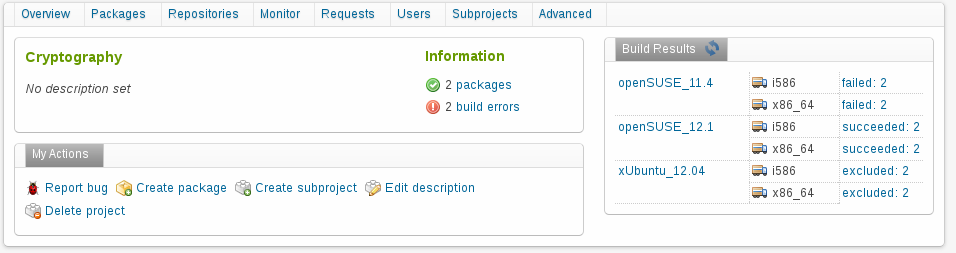
\includegraphics[width=0.75\textwidth]{image/standard/build/opensuse-project-overview.png}
\caption[مدیریت پروژه‌ها در کارگزار ساخت]{
	مدیریت پروژه به قسمت‌های متفاوتی مانند، مخزن‌ها، زیر پروژه‌ها، خصوصیت‌ها و دیگر
	خصوصیت‌های دیگر تشکیل شده است. با استفاده از این سامانه می‌تواند به سادگی
	پروژه‌های ایجاد شده را مدیریت کرد.
}
\label{image/standard/build/opensuse-project-overview}
\end{figure}

به این نکته اشاره شد که هر کاربر نمی‌تواند خارج از پروژه خانه پروژه دیگری داشته
باشد اما به این معنی نیست که کاربر تنها می‌تواند یک پروژه داشته باشد. در این
کارگزار از مفهوم زیرپروژه نیز حمایت می‌شود. هر پروژه می‌تواند از زیر پروژه‌های
متفاوتی ایجاد شده باشد و به همین ترتیب هر زیر پروژه می‌تواند زیرپروژه‌های خاص
خود را داشته باشد. تمام پروژه‌ها و زیر پروژه‌ها به صورت یکسان مدیریت می‌شوند از
نظر کاربردی و امکانات هیچ تفاوتی با یکدیگر ندارد. استفاده از این مفهوم در این
کارگزار تنها برای مدیریت پروژه‌های ایجاد شده بوده و کار برد دیگر ندارد. از این
رو نه تنها کارگزار بلکه کابران می‌توانند تنها با دیدن مسیر هر بسته تعیین کنند که
این بسته به وسیله چه کسی ایجاد شده است.

بر این اساس می‌توان گفت پیش از ایجاد مستند‌های فنی در این کارگزار ساخت می‌بایست
یک فرآیند ابتدایی را برای آماده سازی کارگزار انجام داد. این فرآیند را می‌توان به
صورت مراحل زیر مرتب کرد.

\begin{itemize}
  \item تعیین مخزن‌ها\LTRfootnote{Repository}
  \item اضافه کردن کد برنامه\LTRfootnote{Source code}
  \item تعیین نپشته‌های ایجاد\LTRfootnote{Build Script}
\end{itemize}

همانگونه که اشاره شده هر مخزن معادل با یک سیستم‌عامل است که بسته‌های ایجاد شده
به منظور نصب و راه اندازی به روی آن ایجاد می‌شوند و در نهایت در مسیرهای مناسب
برای همان سیستم‌عامل ساماندهی می‌شوند. از این رو در فرایند تعیین مخزن کافی است
که سیستم‌های عامل مقصد برای پروژه را تعیین کرد. در شکل 
\ref{image/standard/build/opensuse-project-repository}
نمای کلی مدیریت مخزن نمایش داده شده است.

\begin{figure}
\centering
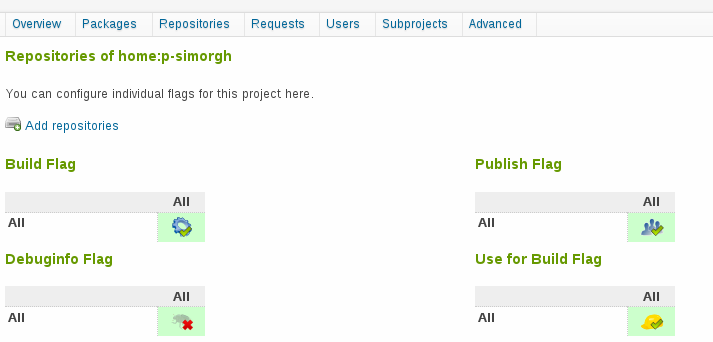
\includegraphics[width=0.75\textwidth]{image/standard/build/opensuse-project-repository.png}
\caption[]{}
\label{image/standard/build/opensuse-project-repository}
\end{figure}

گرچه تولید مستند فنی مستقل از سیستم‌های عامل مورد استفاده است اما در حالت کلی
نمی‌توان با استفاده از کارگزار ساخت بسته‌های مناسب مستند فنی را بدون در نظر
گرفته سکوهای مورد استفاده ایجاد کرد. درحال حاضر سیستم‌عامل‌های متفاوتی در این
کارگزار ساخت مورد حمایت قرار می‌گیرد که در فهرست زیر آورده شده است:

\begin{itemize}
  \item \lr{openSUSE}
  \item \lr{Debian}
  \item \lr{Fedora}
  \item \lr{RedHat}
  \item \lr{CentOS}
  \item \lr{Mandriva}
  \item \lr{Ubuntu}
\end{itemize}

گرچه بسته مستند فنی برای تمام سیستم‌های متفاوت به صورت یکتا ایجاد و تعریف می‌شود
و حتی مستند‌های ایجاد شده به روی هر سیستم‌عامل قابل انتقال به دیگر سیستم‌های
عامل هستند،اما ممکن است فرآیند نصب این بسته‌های در هر سکو متفاوت باشد.
از این رو فرآیند ساخت بسته مستند فنی برای هر سکو متفاوت بوده و از اصول خاص
تعریف شده در سکوی مورد نظر ایجاد می‌شود..

در گام بعد کد منبع بسته نرم افزاری برای کارگزار ساخت تعیین شود. معمولا کد منبع
برای هر سیستم نرم‌افزاری به صورت یک پرونده فشرده به پروژه اضافه می‌شود اما در
برخی موارد از چندین پرونده فشرده برای این منظور استفاده می‌شود.

فرآیند ساخت سیستم‌های نرم‌افزاری در قالب یک بسته نرم‌افزاری در این کارگزار
مدیریت می‌شود. هر بسته نرم‌افزاری شامل تعداد دلخاهی کد منبع است که در کنار
یکدیگر ترجمه شده و سیستم نرم‌افزاری را ایجاد می‌کنند. استفاده از واژه بسته
نرم‌افزاری برای مدیریت یک سیستم نرم‌افزاری و کدهای منبع آن به این معنی نیست که
نتیجه ایجاد یک سیستم نرم‌افزاری تنها می‌تواند به یک بسته منجر شود بلکه در اقلب
موارد نتیجه ساخت سیستم‌های نرم‌افزاری چندی بسته خواهد بود. در ادامه این بخش
منظور از بسته همان مفهومی است که در کارگزار ساخت استفاده می‌شود و در سایر موارد
به آن اشاره خواهد شد.

دور از انتظار نیست که نتیجه ایجاد یک بسته منجر به ایجاد بسته‌های نرم‌افزاری
متفاوتی باشد که یکی از آنها مستند فنی سیستم است. به هر حال در کارگزار ساخت این
حالت پیش بینی شده و امکان ایجاد بسته‌های نرم‌افزاری متفاوت مبتنی بر یک کد منبع
فراهم شده است.

کارگزار ساخت توانایی مدیریت بسته‌های نرم‌افزاری را نیز فراهم کرده است. از این رو
برای هر بسته یک سری ابزار مدیریت فراهم شده است که کاربر با استفاده از آن
می‌تواند به سادگی بسته‌های معرفی شده در سیستم را مدیریت کند. در شکل 
\ref{image/standard/build/opensuse-project-package} ابزارهای موجود برای مدیریت
یک بسته نمایش داده شده است. مهمترین توانایی‌های ایجاد شده برای مدیریت یک بسته در
فهرست زیر آورده شده است:

\begin{itemize}
  \item گزارش حالت کلی بسته
  \item مدیرت کد منبع
  \item مدیریت تقاضا‌ها برای یک بسته
\end{itemize}

در گزارش کلی ایجاد شده برای هر بسته نه تنها تعداد کدهای منبع بلکه تعداد ساخت‌های
موفقیت آمیز، تعداد خطاها، حالت ایجاد بسته برای هر مخزن و سایر موارد دیگر نمایش
داده می‌شود. با استفاده از مدیریت تقاضاها می‌تواند تعیین کرد که نیازهای کاربران
بسته چیست و برای برطرف کردن این نیازها برنامه ریزی کرد.

\begin{figure}
\centering
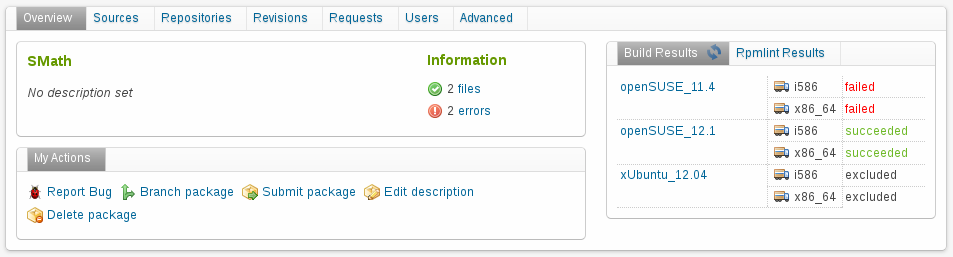
\includegraphics[width=0.75\textwidth]{image/standard/build/opensuse-project-package.png}
\caption[برگه مدیریت پرونده‌ها در کارگزار ساخت \lr{OpenSUSE}]{
	توصیف بسته
}
\label{image/standard/build/opensuse-project-package}
\end{figure}

کارگزار ساخت بسته‌های نرم‌افزاری را مبتنی بر کدهای منبعی ایجاد می‌کند که در بسته
تعریف شده‌اند. گرچه بارگزاری کد منبع به صورت دستی در این کارگزار ممکن است اما
استفاده از سرویس‌های کد منبع روش‌های مناسب‌تری برای این کار فراهم کرده است. برای
نمونه حالتی را فرض کنید که نیاز به دریافت کد منبع از یک سرویس کنترل نسخه باشد و
یا حالتی که در آن می‌بایست پیش از ترجمه برنامه‌ها تغییرات خاصی در آنها ایجاد
شود. در سرویس‌های کد منبع این موارد پیش‌بینی شده و ابزارهای مناسبی برای مدیریت
کدهای منبع ایجاد شده است.

سرویس‌های کد منبع در حقیقت دسته‌ای از وظایف است که کارگزار ساخت پیش از آغاز
فرآیند ساخت آنها را اجرا می‌کند. سرویس‌های کد منبع می‌تواند از دانلود کد منبع تا
اعمال \lr{Patch} به روی کدهای منبع متفاوت باشد. کارگزار ساخت تنها زمانی فرآيند
ایجاد را اجرا می‌کند که تمام سرویس‌های کد منبع به صورت کامل و بدون اشکال اجرا
شود.

علاوه بر کدهای منبع، نپشته‌های مورد استفاده در ساخته بسته‌های نرم‌افزاری نیز
باید به عنوان کد منبع در کارگزار بارگزاری شود. کارگزار ساخت با استفاده از این
بپشته‌ها بسته‌های نرم‌افزاری را ایجاد و در مخزن‌های مربوطه بارگزاری می‌کند.
گرچه نپشته‌های ساخت می‌بایست از استانداردهای خاص برای ایجاد بسته استفاده کنند
اما این کارگزار از قالب‌های متفاوتی برای ایجاد بسته‌ها استفاده می‌کند. یک روش
مناسب برای ایجاد بسته‌ها استفاده از برنامه‌های \lr{spec} است که در مدیریت
بسته‌های کلاه قرمز معرفی شده است. 

در این روش علاوه بر کدهای منبع، پرونده‌های \lr{spec} برای ایجاد بسته‌های
نرم‌افزاری بارگزار می‌شود و در نهایت کارگزار ساخت با استفاده از همین کدها
بسته‌های نرم‌افزاری ار ایجاد می‌کند. کارگزار برای ایجاد بسته‌های نرم افزاری
توزیع \lr{OpenSUSE} از این روش به صورت پیش فرض استفاده می‌کند از این رو در این
بخش تنها همین روش برای ایجاد بسته‌ها مورد استفاده قرار خواهد گرفت.

در اینجا تنها فرآیند ساخته بسته‌های مستند فنی برای توزیع \lr{OpenSUSE} مورد بحث
قرار می‌گیرد که در و همانطور که اشاره شد برای ایجاد بسته مستند فنی از کدهای
\lr{spec} استفاده خواهد شد.

برای نمونه فرض کنید که بسته مورد نظر، \lr{SMath}‌ باشد که در بخش پیش مورد بحث
قرار گرفت. برای ایجاد مستند فنی این بسته با استفاده از این کارگزار در پروژه خانه
ابتدا باید یک بسته ایجاد شود. نام این بسته را نیز همنام با بسته نرم‌افزاری در
نظر گرفته می‌شود. در گام بعد کد منبع به صورت دستی بارگزاری می‌شود. با تعیین
نپشته‌های \lr{spec} کارگزار ساخت فرآیند ساخت بسته را اجرا خواهد کرد و بسته‌های
ایجاد شده را در مخزن‌ها قرار می‌دهد.

\subsection{بسته مستقل}

کارگزار ساخت \lr{OpenSUSE} توانایی اجرای چندین پرونده \lr{spec} را در هر بسته
فراهم کرده است از این رو استفاده از پرنده‌های \lr{spec} برای کارهای متفاوت نه
تنها اشکالی را ایجاد نمی‌کند بلکه به عنوان یک مزیت تلقی می‌شود. گرچه استفاده از
\lr{spec} متفاوت به صورت دستی منجر به ناهماهنگی و سربار در فرآیند ساخت می‌شود
اما در کارگزار ساخت منجر به واضح بودن فرآیندهای ساخت و سادگی آنها می‌شود.

در اینجا نیز مانند روشی که در \lr{RPM} دنبال شد، یک پرونده \lr{spec} ایجاد
می‌شود و فرآیند ساخت بسته به صورت کامل در آن تشریح می‌شود. این پرونده تمام اصول
تعریف شده در \lr{RPM} را در برداشته و از همان روش برای ایجاد بسته‌های نرم افزاری
استفاده می‌کند.

اما نکته‌ای که باید همواره در استفاده از \lr{spec} در کارگزار ساخت مورد توجه قرا
گیرد تعیین بسته‌هایی است که در فرآیند ساخت مورد نیاز است. کارگزار همواره یک
ماشین مجازی را برای ایجاد بسته‌ها ایجاد می‌کند و فرآیند ساخت را مبتی بر آن انجام
می‌دهد. این ماشین مجازی با استفاده از حداقل بسته‌های مورد نیاز بارگزاری می‌شود
از این رو نیاز است که بسته‌ها و ابزارهای مورد نیاز در فرآیند ساخت تعیین شود.

گرچه تعیین بسته‌های مورد نیاز در فرآیند ساخت ممکن است در دید نخست دشوار به نظر
برسد اما این کار با استفاده از \lr{spec} به سادگی قابل انجام است. در این پرونده
با استفاده از برچسب \lr{BuildRequires} می‌توان تمام بسته‌های مورد نیاز برای
فرآیند ساخت را تعیین کرد. این برچسب در قسمت خوصیت‌های عمومی \lr{spec} قرار
می‌گیرد. برای نمونه اگر در فرآیند ساخت نیاز به استفاده از بسته نرم‌افزار \lr{A}
باشد با اضافه کردن کد زیر به پرونده \lr{spec} می‌توان از نصب بودن این بسته پیش
از آغاز شدن فرآیند ساخت اطمینان حاصل کرد.

\begin{latin}
\lstset{language=C++}
\begin{lstlisting}[frame=single]
BuildRequires: A
\end{lstlisting}
\end{latin}

بدیهی است که در فرآیند ساخت مستند فنی نیاز به استفاده از ابزار \lr{Doxygen} است.
از این رو دور از انتظار نیست که در پیش از آغاز فرایند ساخت نیاز به نصب و راه
اندازی این بسته باشد.

نکته‌ای که باید در نظر داشت این است که ممکن است خود ابزارهای مورد نیاز در فرآیند
نصب نیز به بسته‌های دیگری برای اجرا نیاز داشته باشند! در این حالت چه باید کرد؟
کارگزار ساخت فرآیند نصب بسته‌های مورد نیاز را با استفاده از مدیریت بسته‌های
مانند مدیریت بسته‌های کلاه قرمز یا \lr{RPM} انجام می‌دهد، بنابراین سیستم به صورت
خودکار نه تنها بسته مورد نیاز بلکه تمام بسته‌های مورد نیاز دیگر ار نصب خواهد
کرد.

از دیگر بسته‌های مورد نیزا در فرآیند ساخت می‌توان به \lr{texlive} اشاره کرد.
\lr{Doxyge} با استفاده از ابزارهای معرفی شده در این بسته رابطه‌های ریاضی را
ایجاد می‌کند و در نهایت مستند فنی در قالب چاپی را نیز با همین ابزار ایجاد
می‌کند. اما خود بسته \lr{Doxygen} به این بسته وابسته نیست، بنابر این اگر این
بسته به عنوان بسته مورد نیاز در فرآیند ایجاد معرفی نشود، فرآیند ایجاد مستند فنی
با مشکل روبرو خواهد شد.

در گفتارهای پیشین ابزارهای متفاوتی به عنوان ابزارهای مورد استفاده در
\lr{Doxygen} معرفی شده است که می‌تواند در فرآیند ساخت مورد استفاده قرار گیرد. از
این رو پیش از فرآیند ساخت می‌بایست از نصب بودن آنها اطمینان حاصل کرد. البته
استفاده از این بسته‌ها به تنظیم‌های موجود در پرونده پیکره بندی مستند فنی
وابسته‌ است.

برای نمونه در ایجاد مستند فنی \lr{SMath} ابزارهای مورد نیاز به صورت زیر تعیین
شده است که شامل تمام ابزارهای مورد نیاز برای ساخت یک مستند فنی کامل است.


% TODO: maso 1391: تعیین بسته‌های مورد نیاز
% برای نصب کامل یک سیستم به بسته‌های متفاوتی نیاز است که از آنها در ترسیم و یا
% سازماندهی کردن مستند استفاده می‌شود. از این رو نیاز است که این بسته‌ها به صورت
% کامل و دقیق برای مستند سازی تعیین شود.

\begin{latin}
\lstset{language=C++}
\begin{lstlisting}[frame=single]
BuildRequires: texlive texlive-bin texlive-fonts-extra texlive-xetex 
graphviz doxygen
\end{lstlisting}
\end{latin}

با ایجاد این تغییرها و اضافه کردن پرونده \lr{spec} سرور ساخت فرآیند ایجاد را
زمان بندی کرده و در موقعیت مناسب اجرا می‌کند. در نهایت نتیجه به دست آمده در
فهرست بسته‌های موجود مخزن‌های نرم‌افزاری ایجاد شده قرار می‌گیرد و کاربران می‌توانند
از آنها استفاده کنند.

\subsection{زیر بسته مستند فنی}

همانند روش زیر بسته که در بخش  \lr{RPM} معرفی شد، در اینجا نیز می‌توان با
استفاده از یک پرونده \lr{spec} نه تنها برنامه‌های ایجرایی بلکه مستندهای فنی را
نیز ایجاد کرد. تنها تفاوت مهمی که در اینجا نیاز است تعیین بسته‌هایی است که در
فرآیند ساخت مورد نیاز است.

بسته‌های مورد نیاز در فرایند ساخت ممکن است برای هر زیر بسته متفاوت باشد با این
وجود تمام بسته‌های مورد نیاز در بخش اصلی معرفی می‌شود. از این رو برای ایجاد زیر
بسته مستند فنی می‌بایست پیش از هر چیز ابزارهای مورد نیاز را تعیین کرد. در تکه کد
زیر روش تعیین ابزارهای مورد نیاز آورده شده است.

\begin{latin}
\lstset{language=C++}
\begin{lstlisting}[frame=single]
BuildRequires: gcc make automake libqt4-devel ... doxygen ...
\end{lstlisting}
\end{latin}

با اضافه کردن ابزارها و بارگزار پرونده \lr{spec}، کارگزار علاوه بر ایجاد
بسته‌های نرم‌افزار بسته مستند فنی را نیز ایجاد خواهد کرد.
